\usepackage{pgfplots}
\pgfplotsset{compat=1.17}
\usepackage{adjustbox}
\usepackage{float}
\usepackage{caption}

\usepackage{xcolor}
\definecolor{codegray}{RGB}{128,128,128}
\definecolor{line_color}{RGB}{0,51,160}
\definecolor{mark_color}{RGB}{177,2,2}
\definecolor{avg_color}{RGB}{255, 163, 0}

\usepackage{listings}
\lstset{
  language=C++, % choose the language of the code
  basicstyle=\ttfamily\footnotesize,
  numberstyle=\tiny\color{codegray},
  numbers=left, % where to put the line-numbers
  numbersep=5pt,
}

%For getting the average of a parametric equation using gnuplot
\usepackage{shellesc}

\newcounter{PolynomialID}
\newcommand\getPolynomialID{polynomial\thePolynomialID}
\newcommand{\polynomial}[3][0.9\columnwidth]{
  \begin{figure}[H]
    \begin{center}
      \begin{adjustbox}{width = #1}
        \begin{tikzpicture}
          \begin{axis}[
              axis lines=center,
              xmin=-6, xmax=6,
              ymin=-6, ymax=6,
              xtick={-5,-4,...,5},
              ytick={-5,-4,...,5},
              domain = -6:6,
              restrict y to domain=-20:20,
              xtick distance=1,
              ytick distance=1,
              grid=major,
              grid style = {solid},
              yticklabels={,,},
              xticklabels={,,},]
            \addplot[id=\getPolynomialID,samples=100,line_color,style={thick},smooth] {#2};
          \end{axis}
        \end{tikzpicture}
      \end{adjustbox}
    \end{center}
    \caption*{#3}
  \end{figure}
  \stepcounter{PolynomialID}
}

\newcounter{MarkID}
\newcommand\getMarkID{mark\theMarkID}

\newcounter{WaveID}
\newcommand\getWaveID{wave\theWaveID}
\newlength{\wavewidth}
\newcommand{\waveform}[4][0.9\columnwidth]{% args: size, function(x), marks, caption
  \setlength{\wavewidth}{#1}
  \begin{figure}[H]
    \begin{center}
      \begin{tikzpicture}
        \begin{axis}[
            axis lines=center,
            tick pos = right,
            width = \wavewidth,
            height = 0.19\wavewidth,
            xmin=0, xmax=4,
            ymin=-2, ymax=2,
            xtick={1,2,3},
            ytick={-1,0,1},
            domain = 0:4,
            restrict y to domain=-4:4,
            xtick distance=1,
            ytick distance=1,
            grid=major,
            grid style = {solid},
            yticklabels={,,},
            xticklabels={,,},]
          \addplot[id=\getWaveID,samples=400,line_color,style={thick},smooth] function{#2};
          \ifnum#3>0
            \addplot[id=\getMarkID,samples=#3,mark_color,only marks, mark=*] function{#2};
            \stepcounter{MarkID}
          \fi
        \end{axis}
      \end{tikzpicture}
    \end{center}
    \caption*{#4}
  \end{figure}
  \stepcounter{WaveID}
}

\newcommand{\criticalFrequency}[2][0.9\columnwidth]{% args: size, caption
  \setlength{\wavewidth}{#1}
  \begin{figure}[H]
    \begin{center}
      \begin{tikzpicture}
        \begin{axis}[
            axis lines=center,
            tick pos = right,
            width = \wavewidth,
            height = 0.19\wavewidth,
            xmin=0, xmax=4,
            ymin=-2, ymax=2,
            xtick={1,2,3},
            ytick={-1,0,1},
            domain = 0:4,
            restrict y to domain=-4:4,
            xtick distance=1,
            ytick distance=1,
            grid=major,
            grid style = {solid},
            yticklabels={,,},
            xticklabels={,,},]
          \addplot[id=\getWaveID,samples=400,line_color,style={thick},smooth] function{cos(2*2*pi*x + 0.5) - sin(2*2*pi*x) * tan(0.5)};
          \stepcounter{WaveID}
          \addplot[id=\getWaveID,samples=400,mark_color,style={thick},smooth] function{cos(2*2*pi*x + 0.8) - sin(2*2*pi*x) * tan(0.8)};
          \stepcounter{WaveID}
          \addplot[id=\getWaveID,samples=400,avg_color,style={thick},smooth] function{cos(2*2*pi*x + 0.2) - sin(2*2*pi*x) * tan(0.2)};
          \stepcounter{WaveID}
          \addplot[only marks, black, mark=*] coordinates
            {(0.23,-1.1) (0.48,1.1)
              (0.73,-1.1) (0.98,1.1)
              (1.23,-1.1) (1.48,1.1)
              (1.73,-1.1) (1.98,1.1)
              (2.23,-1.1) (2.48,1.1)
              (2.73,-1.1) (2.98,1.1)
              (3.23,-1.1) (3.48,1.1)
              (3.73,-1.1) (3.98,1.1)};
        \end{axis}
      \end{tikzpicture}
    \end{center}
    \caption*{#2}
  \end{figure}
}

\newcounter{PhasorID}
\newcommand\getPhasorID{phasor\thePhasorID}
\newcommand\genPhasorTableFilename{\jobname.\getPhasorID.table}

\newcommand{\calcPhasorAverage}[1][\genPhasorTableFilename]{% arg: filename
  \ShellEscape{gnuplot -e "stats '#1' using 1; x_avg = STATS_mean; stats '#1' using 2; y_avg = STATS_mean; set print '#1.avg'; print x_avg, y_avg"}%
}

% args: size, equation(t), period, marks, caption
% mark being 0 turns off the average indicator, 1 only average indicator, > 1 marks & average
\newcommand{\phasor}[5][0.9\columnwidth]{
  \begin{figure}[H]
    \begin{center}
      \begin{adjustbox}{width = #1}
        \begin{tikzpicture}
          \begin{axis}[
              axis lines=center,
              xmin=-4, xmax=4,
              ymin=-4, ymax=4,
              xtick={-3,-2,...,3},
              ytick={-3,-2,...,3},
              xlabel={$\Re$},
              ylabel={$\Im$},
              xtick distance=1,
              ytick distance=1,
              grid=major,
              grid style = {solid},
              yticklabels={,,},
              xticklabels={,,},]
            \addplot gnuplot[parametric,id=\getPhasorID,domain=0:8,samples=1000,line_color,style={thick},smooth,solid, no markers] {
                (#2) * cos((-2 * pi * t) * (#3)),
                (#2) * sin((-2 * pi * t) * (#3))
              };
            \ifnum#4>1
              \addplot gnuplot[parametric,id=\getMarkID,domain=0:4,samples=#4,mark_color,only marks, mark=*] {
                  (#2) * cos((-2 * pi * t) * (#3)),
                  (#2) * sin((-2 * pi * t) * (#3))
                };
              \stepcounter{MarkID}
            \fi
            \ifnum#4>0
              \calcPhasorAverage
              \addplot[mark=*,avg_color] table {\genPhasorTableFilename.avg};
            \fi
          \end{axis}
        \end{tikzpicture}
      \end{adjustbox}
    \end{center}
    \caption*{#5}
  \end{figure}
  \stepcounter{PhasorID}
}

\newcommand{\unitCircle}[1][0.9\columnwidth]{
  \begin{figure}[H]
    \begin{center}
      \begin{adjustbox}{width = #1}
        \begin{tikzpicture}
          \begin{axis}[
              axis lines=center,
              axis equal,
              enlargelimits,
              xmin=-1, xmax=1,
              ymin=-1, ymax=1,
              xlabel={$\Re$},
              ylabel={$\Im$},
              ticks = none,
              thick]
            \draw[radius = 1] (0,0) circle;
            \draw[avg_color] (0,0) -- (0.125,0) arc[start angle=0, end angle=45,radius=0.125] node[avg_color, right]{\theta};
            \draw[black] (0,0) -- (45:1) node[black, midway, above left]{1} node[black,above right]{$e^{i\theta}$};
            \draw[mark_color] (0,0) -- (0.70710678118,0) node[mark_color, midway, below right]{$cos(\theta)$};
            \draw[line_color] (0.70710678118,0) -- (0.70710678118,0.70710678118) node[line_color, fill = white, midway, right]{$i \cdot sin(\theta)$};
            %this was genuinely the easiest way to draw a dot here
            \addplot[black,mark=*] coordinates {(0.70710678118,0.70710678118)};
          \end{axis}
        \end{tikzpicture}
      \end{adjustbox}
    \end{center}
    \caption*{The Complex Unit Circle}
  \end{figure}
}

\newcounter{SpectrumID}
\newcommand\getSpectrumID{spectrum\theSpectrumID}
\newcommand\genSpectrumTableFilename{\jobname.\getSpectrumID.table}

\newcommand{\genInitSpectrumTable}[4][\genSpectrumTableFilename]{% arg: filename, upper bound, samples, equation(x)
  \ShellEscape{gnuplot -e "set table '#1'; set samples #3; set dummy x; plot [x=0:#2] (#4);"}%
  \ShellEscape{perl ../common/fft.pl '#1' #2}%
}
% arg: size, seconds, window, samples, equation(x), caption
\newcommand{\fourierSpectrum}[6][0.9\columnwidth]{
  \begin{figure}[H]
    \begin{center}
      \begin{adjustbox}{width = #1}
        \begin{tikzpicture}
          \begin{axis}[
              axis lines = left,
              tick align = inside,
              xmin=0, xmax=#3,
              ymin=0, ymax=1,
              xtick distance = 1,
              ytick distance = 1,
              ytick={0.25,0.5,0.75},
              grid=major,
              grid style = {solid},
              xlabel = {Frequency Bin},
              ylabel = {Magnitude},
              x label style={at={(axis description cs:0.5,-0.1)},anchor=north},
              y label style={at={(axis description cs:-0.1,.5)},anchor=south},]
            \genInitSpectrumTable{#2}{#4}{#5}
            \ifnum#4>64
              \addplot[mark=none,line_color,smooth,thick,fill] table {\genSpectrumTableFilename};
            \else
              \addplot[only marks, mark=*,line_color] table {\genSpectrumTableFilename};
            \fi
          \end{axis}
        \end{tikzpicture}
      \end{adjustbox}
    \end{center}
    \caption*{#6}
  \end{figure}
  \stepcounter{SpectrumID}
}

\newcommand{\rootsOfUnity}[1][0.9\columnwidth]{
  \begin{figure}[H]
    \begin{center}
      \begin{adjustbox}{width = #1}
        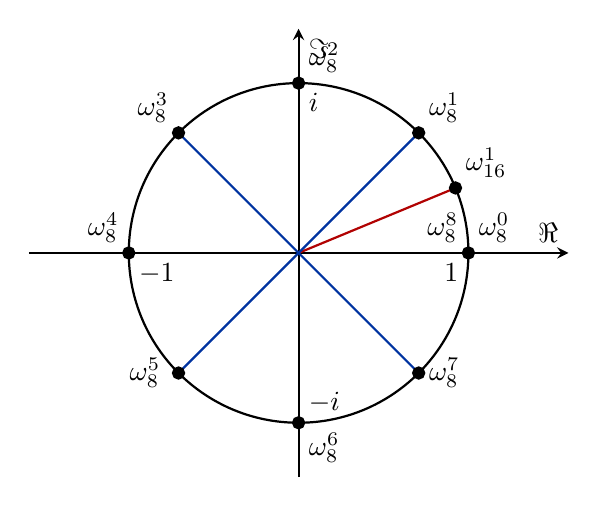
\begin{tikzpicture}
          \begin{axis}[
              axis lines=center,
              axis equal,
              enlargelimits,
              xmin=-1, xmax=1,
              ymin=-1.1, ymax=1.1,
              xlabel={$\Re$},
              ylabel={$\Im$},
              ticks = none,
              thick]
            \draw[radius = 1] (0,0) circle;
            \draw[mark_color] (0,0) -- (0.92387953251,0.38268343236);
            \addplot[black,mark=*] coordinates {(0.92387953251,0.38268343236)} node[above right] {$\omega_{16}^1$};
            \draw[line_color] (0,0) -- (0.70710678118,0.70710678118);
            \draw[line_color] (0,0) -- (-0.70710678118,0.70710678118);
            \draw[line_color] (0,0) -- (-0.70710678118,-0.70710678118);
            \draw[line_color] (0,0) -- (0.70710678118,-0.70710678118);
            \addplot[black,mark=*] coordinates {(1,0)} node[above right] {$\omega_8^0$} node[above left] {$\omega_8^8$} node[below left] {$1$};
            \addplot[black,mark=*] coordinates {(0.70710678118,0.70710678118)} node[above right] {$\omega_8^1$};
            \addplot[black,mark=*] coordinates {(0,1)} node[above right] {$\omega_8^2$} node[below right] {$i$};
            \addplot[black,mark=*] coordinates {(-0.70710678118,0.70710678118)} node[above left] {$\omega_8^3$};
            \addplot[black,mark=*] coordinates {(-1,0)} node[above left] {$\omega_8^4$} node[below right] {$-1$};
            \addplot[black,mark=*] coordinates {(-0.70710678118,-0.70710678118)} node[left,xshift=-0.1cm] {$\omega_8^5$};
            \addplot[black,mark=*] coordinates {(0,-1)} node[below right] {$\omega_8^6$} node[above right] {$-i$};
            \addplot[black,mark=*] coordinates {(0.70710678118,-0.70710678118)} node[right] {$\omega_8^7$};
          \end{axis}
        \end{tikzpicture}
      \end{adjustbox}
    \end{center}
    \caption*{The 8th Roots of Unity and First 16th Root of Unity}
  \end{figure}
}

\newcounter{ButterflyID}
\newcommand\getButterflyID{butterfly\theButterflyID}
\newcommand\genButterflyFilename{\jobname.\getButterflyID.out}

\newcommand{\genButterflyDIF}[2][\genButterflyFilename]{% arg: filename, samples
  \ShellEscape{perl ../common/butterfly-dif.pl #2 > '#1'}%
}

\usetikzlibrary {arrows.meta}

%args: size
\newcommand{\butterfly}[2][\linewidth]{
  \begin{figure}[H]
    \begin{center}
      \begin{tikzpicture}
        \begin{axis}[
            width = #1,
            axis line style={draw=none},
            tick style={draw=none},
            yticklabels={,,},
            xticklabels={,,},
          ] 
          \genButterflyDIF{#2}
          \input{\genButterflyFilename}
        \end{axis}
      \end{tikzpicture}
    \end{center}
    \caption*{The Cooley-Tukey Radix-2 Decimation-In-Frequency Fast Fourier Transform}
  \end{figure}
  \stepcounter{ButterflyID}
}